\section{Udvælgelse af gestik-par til at skifte musiknummer}
\label{TestresultaterSkiftMusiknummer}
%
Udvælgelsen af hvilket gestik-par, der skal knyttes til at skifte musiknummer foretages på baggrund af testpersonernes begrundelser for til- og fravalg af de foreslåede gestikker. Der fokuseres først på hvilke gestik-par testpersonerne har inddraget i deres top tre rangering og i den forbindelse, om det er muligt at ekskludere nogle gestik-par. Derefter fokuseres der på testpersonernes begrundelser for, hvorfor de har valgt de gestik-par, som de har, hvorunder forbedringsforslag inkluderes, hvis testpersonerne fremsætter nogle. Afsnittet vil afslutningsvist ende ud i hvilket gestik-par, der vælges til at skifte musiknummer.\blankline
%
Få at få et overblik over, hvor ofte de syv forskellige gestik-par individuelt indgår på enten en første-, anden- eller tredjeplads i top tre rangeringen opstilles følgende \autoref{fig:SamletTopTreSkift}. 
%
\begin{figure}[H]
	\centering
	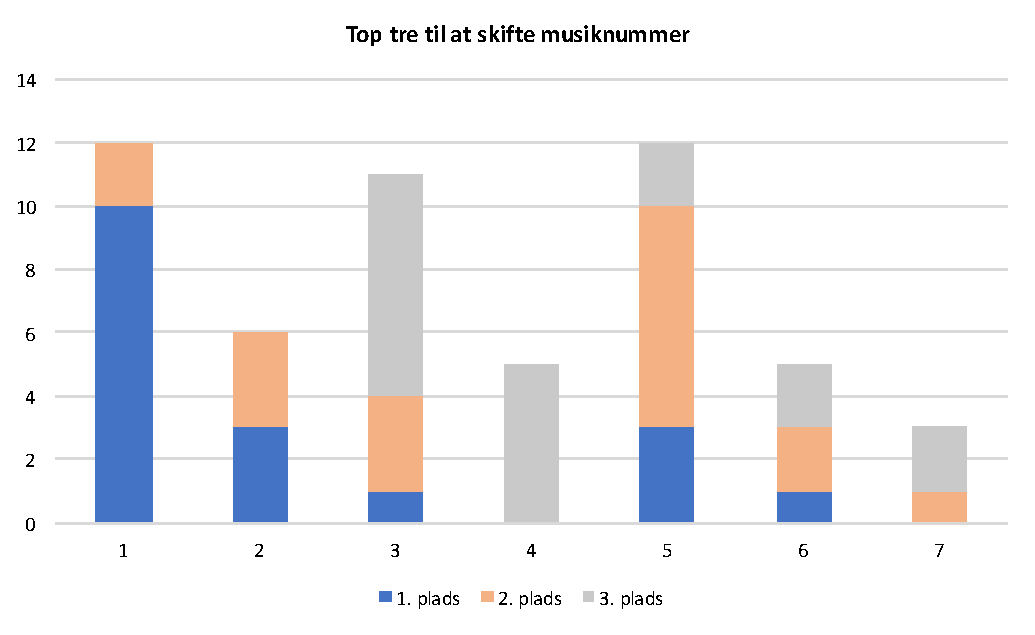
\includegraphics[resolution=300,width=0.9\textwidth]{Test1/DatabehandlingGrafer/TopTreSkift}
	\caption{Søjlediagram over hvordan hvert gestik-par indgår i testpersonernes top tre i forhold til at skifte musiknummer. Data forefindes i \autoref{app:TopTreRangeringSkift}}
	\label{fig:SamletTopTreSkift}
\end{figure}
\noindent
%
På \autoref{fig:SamletTopTreSkift} fremgår det tydeligt, at GP1, GP3 samt GP5 er de tre gestik-par, som uafhængigt af den specifikke plads, indgår flest gange i testpersonernes top tre. Derudover tyder det på, at hverken GP4, GP6 eller GP7 er specielt eftertragtet, da de henholdvis kun indgår fem, fem og tre gange i testpersonernes samlede top tre, jævnfør \autoref{fig:SamletTopTreSkift}. For at vurdere om der er belæg for, at ekskludere et eller flere gestik-par opstilles følgende \autoref{fig:DaarligstGestikSkift}. 
%
\begin{figure}[H]
	\centering
	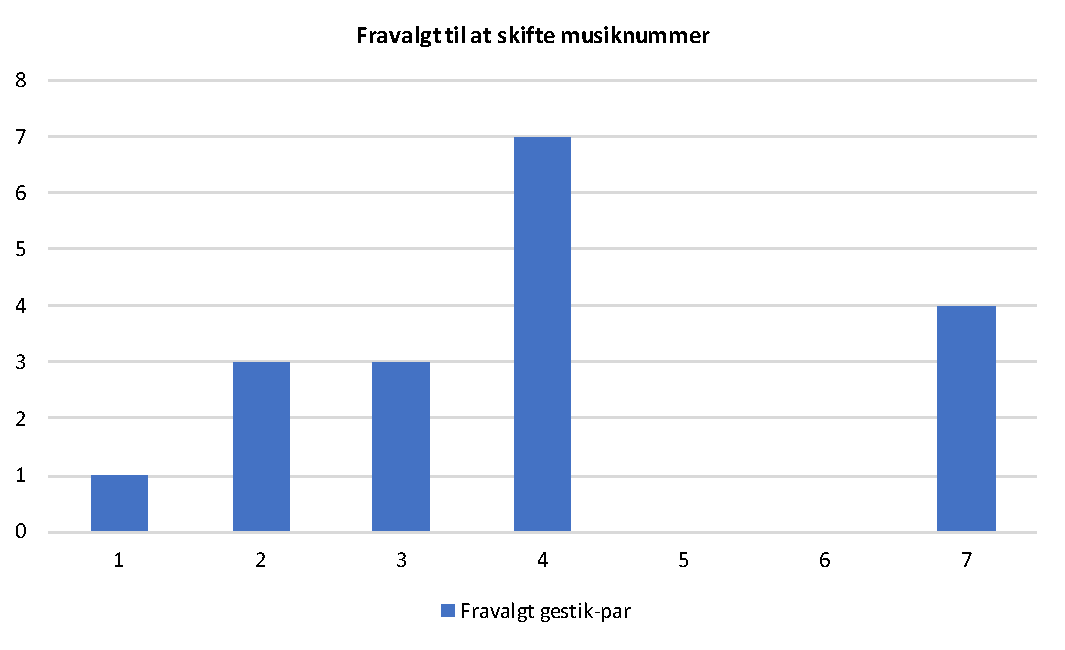
\includegraphics[resolution=300,width=0.9\textwidth]{Test1/DatabehandlingGrafer/FravalgtSkift}
	\caption{Søjlediagram over hvilke gestik-par testpersonerne fravælger i forbindelse med at skifte musiknummer.}
	\label{fig:DaarligstGestikSkift}
\end{figure}
\noindent
%
På \autoref{fig:DaarligstGestikSkift} opsummeres antallet af gange hvert gestik-par fravælges af testpersonerne. Da syv ud af 18 testpersoner har fravalgt GP4 konkluderes det, at testpersonerne ikke bryder sig om GP4, hvorfor GP4 ekskluderes. På \autoref{fig:SamletTopTreSkift} fremgår det, at GP6 kun tildeles én førsteplads og derudover kun indgår to gange på henholdvis en anden- og tredjeplads og selvom GP6 aldrig fravælges af testpersonerne, så vurderes det, at GP6 er overflødig og irrelevant. Der er derfor belæg for at ekskludere GP6. Tilsvarende er gældende for GP7, som kun indgår tre gange i testpersonernes samlede top tre og aldrig tildeles en førsteplads, jævnfør \autoref{fig:SamletTopTreSkift}, og derudover fravælges fire gange, jævnfør \autoref{fig:DaarligstGestikSkift}. Der er derfor belæg for at ekskludere GP7. Selvom GP2 indgår seks gange i den samlede top tre, så ekskluderes dette gestik-par. Det gøres, blandt andet, ud fra et ønske om ikke at gå i mod Bang $\&$ Olufsen's designvalg i forhold til, hvilken retning swipe-bevægelsen skal foretages i for at skifte til det næste musiknummer. I \autoref{app:TestresultaterSkiftDaarlig} forefindes en dybere analyse af hvorfor testpersonerne fravælger de gestik-par, som de gør. 

Ekskluderingen af de fire gestik-par medfører, at den efterfølgende analyse vil omhandle testpersonernes begrundelser for at vælge GP1, GP3 samt GP5.
%
\subsection{Testpersonernes begrundelse for valg af gestik-par 1}
\label{TestresultaterValgAfGestikkerBegrundelseGP1Skift}
%
Med udgangspunkt i \autoref{fig:SamletTopTreSkift} tildeles GP1 en førsteplads af 10 testpersoner, en andenplads af to testpersoner og aldrig en tredjeplads. GP1 illustreres på \autoref{fig:GestikPar1Skift}. De testpersoner, som har tildelt GP1 en førsteplads, begrunder det ud fra en kombination af følgende egenskaber: 
%
\begin{multicols}{3}
    \begin{itemize}
        \item Foretrækker dynamik
        \item Naturlig
        \item Giver mening
        \item Simpel
        \item Intuitiv
        \item Logisk
        \item Enkel
        \item Nem at udføre
        \item Nem at forstå
\end{itemize}
\end{multicols}
\noindent
%
Derudover relaterer testpersonerne GP1 til hvordan der normaltvist interageres med tablets og smartphones, hvilket indikerer at de har erfaring med swipe-bevægelser. Ydermere påpeges det, at der i GP1 ikke er et besværligt håndtegn, som skal gengives for at skifte musiknummer.
%
\begin{figure}[H]
	\centering
	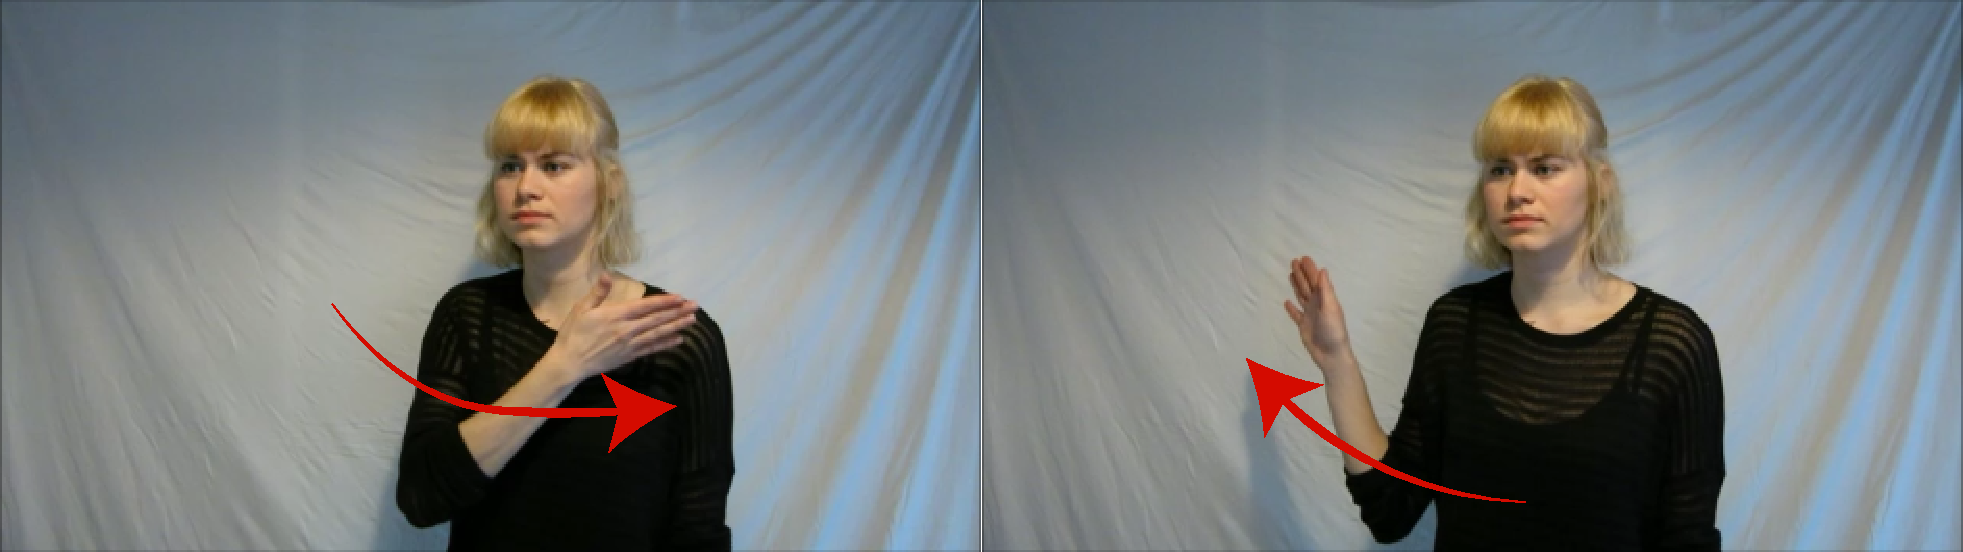
\includegraphics[resolution=300,width=0.9\textwidth]{Test1/Gestik-par/Gestik1_SkiftSang}
	\caption{Illustration af gestik-par 1; swipe fra højre mod venstre for at skifte til det næste musiknummer og fra venstre mod højre for at skifte til det forrige musiknummer.}
	\label{fig:GestikPar1Skift}
\end{figure}
\noindent
%
Sammenholdes udtalelserne fra de 10 testpersoner med hvad de rent faktisk gør så er der fire, som ikke formår at udføre bevægelsen i GP1 konsekvent. TP1 alternerer mellem at gengive GP1 og GP5, når testpersonen generelt referer til en swipe-bevægelse, men når testpersonen afslutningsvist gengiver sine fortrukne gestikker, så gengives GP1. I HENVISNING forefindes videomateriale for den pågældende situation. I begyndelsen foretrækker TP7 GP7, hvorefter testpersonen ræsonnerer sig frem til, at det istedet er GP1 testpersonen foretrækker. Dog med forbehold for at TP7 foretrækker en mindre bevægelse. Når TP7 afslutningsvist gengiver sine fortrukne gestikker, så gengives GP5, dog i den modsatte retning. Når TP15 taler om GP2, så gengiver testpersonen GP1 og når testpersonen opfordres til at prøve gestikkerne til musik så gengives de med både højre og venstre hånd, hvor begge bevægelser er modsat af bevægelsen i GP1. Afslutningsvist er det dog GP1, som TP15 gengiver. Samme tendens forefindes ved TP16, som først gengiver GP1, hvorefter der afslutningsvist forklares og gengives bevægelsen svarende til GP2. Testlederen gengiver GP1 for, at være sikker på hvad TP16 foretrækker, hvor testpersonen giver udtryk for, at det er sådan det skal være. I begge tilfælde, så er der indikationer af, at både TP15 og TP16 er i tvivl om hvilken retning swipe-bevægelsen skal foregå i for at skifte til enten det næste eller forrige musiknummer.

Derudover påpeger TP6 et potentielt problem, som opstår når der skal skiftes tilbage til det forrige musiknummer og ikke for at genspille musiknummeret. Testpersonen er bekymret for, at det bliver nødvendigt at svinge mange gange i luften, for at rent faktisk at skifte til det forrige musiknummer. Det er selvfølgelig en problemstilling, der skal tages højde for, men som det er kendt fra andre musikafspillere; så skiftes der til det forrige musiknummer, hvis det gøres inden for relativt kort tid, derefter genspilles musiknummeret. Det antages derfor at dette ligeledes implementeres i Bang $\&$ Olufsen's fremtidige musikanlæg. 
%
\subsubsection{Forbedringsforslag til gestik-par 1}
\label{TestresultaterValgAfGestikkerForbedringGP1Skift}
%
Af de 10 testpersoner, som har valgt GP1, er der fire testpersoner, som har forbedringsforslag. Ifølge TP2 skal antallet af fingre i swipe-bevægelsen være ligegyldig, da det er bevægelsen, der er essentiel. Det antages derfor at testpersonen formentlig ikke vil have noget imod at benytte GP5 istedet. Testpersonen har tildelt GP5 en andenplads. TP5 foreslår at bevægelsen skal være et "ninja hug", hvor fingrene samles, håndfladen peger opad og bevæges skråt ned fra højre mod venstre for at skifte til det næste musiknummer. For at skifte til det forrige musiknummer, foreslår TP5, igen at fingrene samles med denne gang skal håndfladen pege nedad og bevæges skråt ned fra venstre mod højre. Forbedringsforslaget fra TP5 forefindes i videomaterialet vedlagt HENVISNING. Forbedringsforslaget afvises dog, da bevægelsen bliver stiv og bestemt, hvilket forventes at have en negativ effekt på den sociale accept.

For at undgå det problem som TP6 påpeger, foreslår testpersonen at GP3 benyttes til at skifte til det forrige musiknummer, for at undgå genspilningen. Dette forslag afvises dog, da en opdeling af funktionen potentielt kan gøre det svære at lærer og derudover afviger det fra hvordan tilbage-funktionen normalvist fungerer. 

For at skifte til det næste musiknummer foreslår TP10, at højre hånd føres ind foran kroppen og for at skifte til det forrige musiknummer føres venstre hånd ind foran kroppen. Uanset om det er GP1 eller andre, der anvendes til at skifte musiknummer, så forventes det, at det er muligt at gengive gestikken med begge hænder. Det er derfor uhensigtmæssigt at knytte en bestemt hånd til en bestem retning, hvorfor forbedringsforslaget afvises.     
%
\subsection{Testpersonernes begrundelse for valg af gestik-par 3}
\label{TestresultaterValgAfGestikkerBegrundelseGP3Skift}
% 
Med udgangspunkt i \autoref{fig:SamletTopTreSkift} tildeles GP1 en førsteplads af 10 testpersoner, en andenplads af to testpersoner og aldrig en tredjeplads. GP1 illustreres på \autoref{fig:GestikPar1Skift}. De testpersoner, som har tildelt GP1 en førsteplads, begrunder det ud fra en kombination af følgende egenskaber: 




%
\begin{figure}[H]
	\centering
	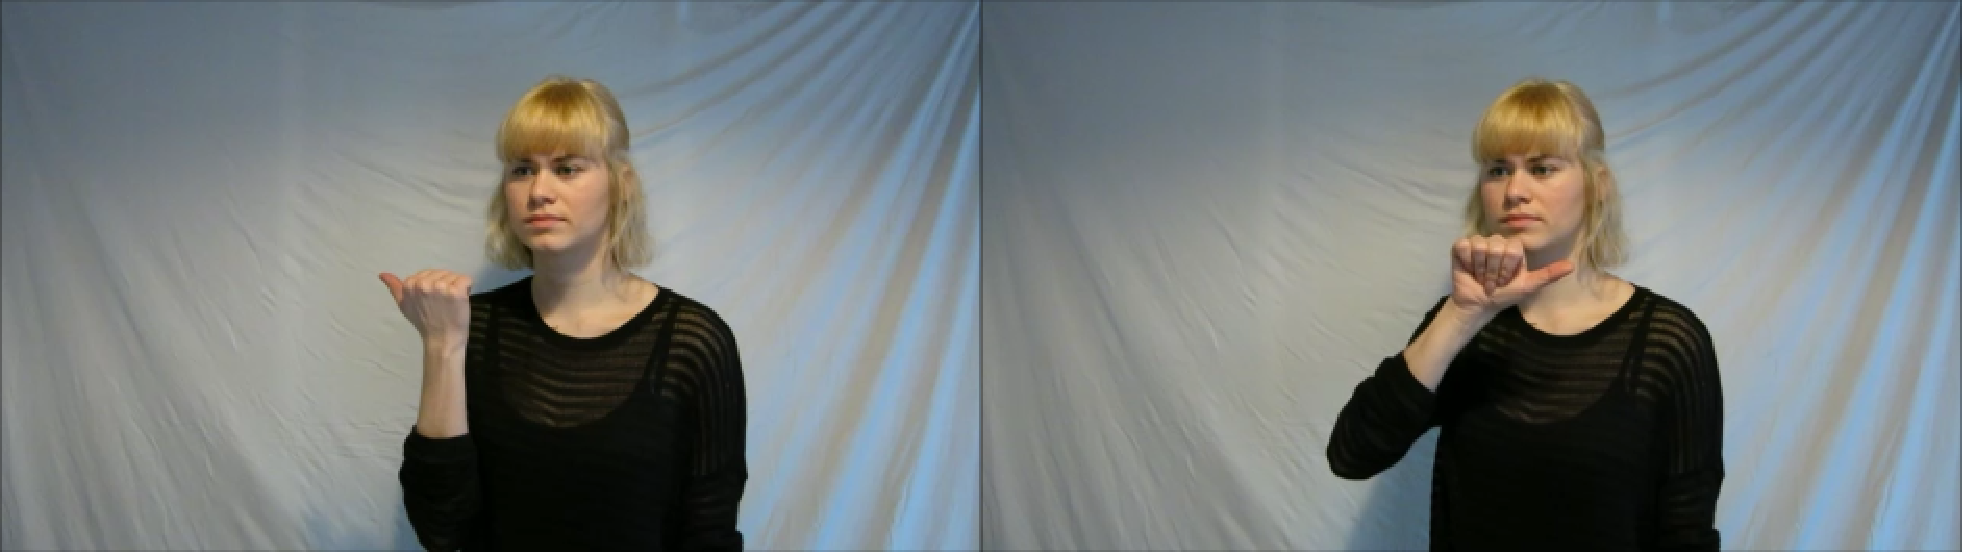
\includegraphics[resolution=300,width=0.9\textwidth]{Test1/Gestik-par/Gestik3_SkiftSang}
	\caption{Illustration af gestik-par 3; tommelfinger peger den retning musiknummeret skal skifte i. Først frem og derefter tilbage til det forrige musiknummer.}
	\label{fig:GestikPar3Skift}
\end{figure}
\noindent
% 
Ud fra \autoref{tab:GestikParITopTreSkiftOversigt} fremgår det, at der kun er én testperson, som har tildelt gestik-par 3 en første plads. Gestik-par 3 illustreres på \autoref{fig:GestikPar3Skift}. Årsagen til at testperson 8 har valgt gestik-par 3 er fordi det er klart og tydeligt hvad der skal gøres. Foruden gestik-par 3 så har testperson 8 rangeret gestik-par 7 på en tredje plads, jævnfør \autoref{tab:GestikParITopTreSkift}, hvilket indikerer at testpersonen foretrækker en lille bevægelsesmængde. Når gestik-par 3 indgår på en anden plads, så er det i to ud af tre tilfælde efter gestik-par 1. Testperson 16 har rangeret gestik-par 3 over gestik-par 7 fordi den er mere diskret. Derudover pointerer testpersonen at de er nemme at udføre samt at det er de eneste to par, hvor der ikke skal en bevægelse til, hvilket ifølge testpersonen er ret smart. At det er nemt at udføre pointerer testperson 6 også. Gestik-par 3 rangeres på en tredje plads syv gange, hvor testperson 2 og testperson 5 har inkluderet parret i top tre enten fordi der ikke var andre, som kunne accepteres eller fordi det var det par, der kom tættest på en tredje plads. Det tyder ligeledes på, at testperson 9 har brugt udelukkelses metoden og i forhold til gestik-par 3 kommenterer testpersonen, at det er en meget lille bevægelse som er nem at overse. Testperson 10 giver udtryk for at årsagen til at gestik-par 3 inkluderes er fordi den er enorm simpel. Testperson 18 foretrækker både sin første og anden plads over gestik-par 3, da de er mere naturlige, men derudover kommenterer testpersonen at gestik-par 3 kan laves forholdvist passivt. Hverken testperson 4 eller testperson 7 forklarer hvorfor de har inkluderet gestik-par 3. 

I og med at der kun er en enkelt testperson, som har rangeret gestik-par 3 på en første plads og at det tyder på at største delen af de andre testpersoner, som har inkluderet gestik-par 3 har gjort det ud fra udelukkelsesmetoden og sammenholdt med \fullref{app:TestresultaterSkiftDaarlig}, hvor tre testpersoner har fravalgt gestik-par 3, så vurderes det at der belæg for at ekskludere gestik-par 3.
%
\subsection{Testpersonernes begrundelse for valg af gestik-par 5}
\label{TestresultaterValgAfGestikkerBegrundelseGP5Skift}
%
%
\begin{figure}[H]
	\centering
	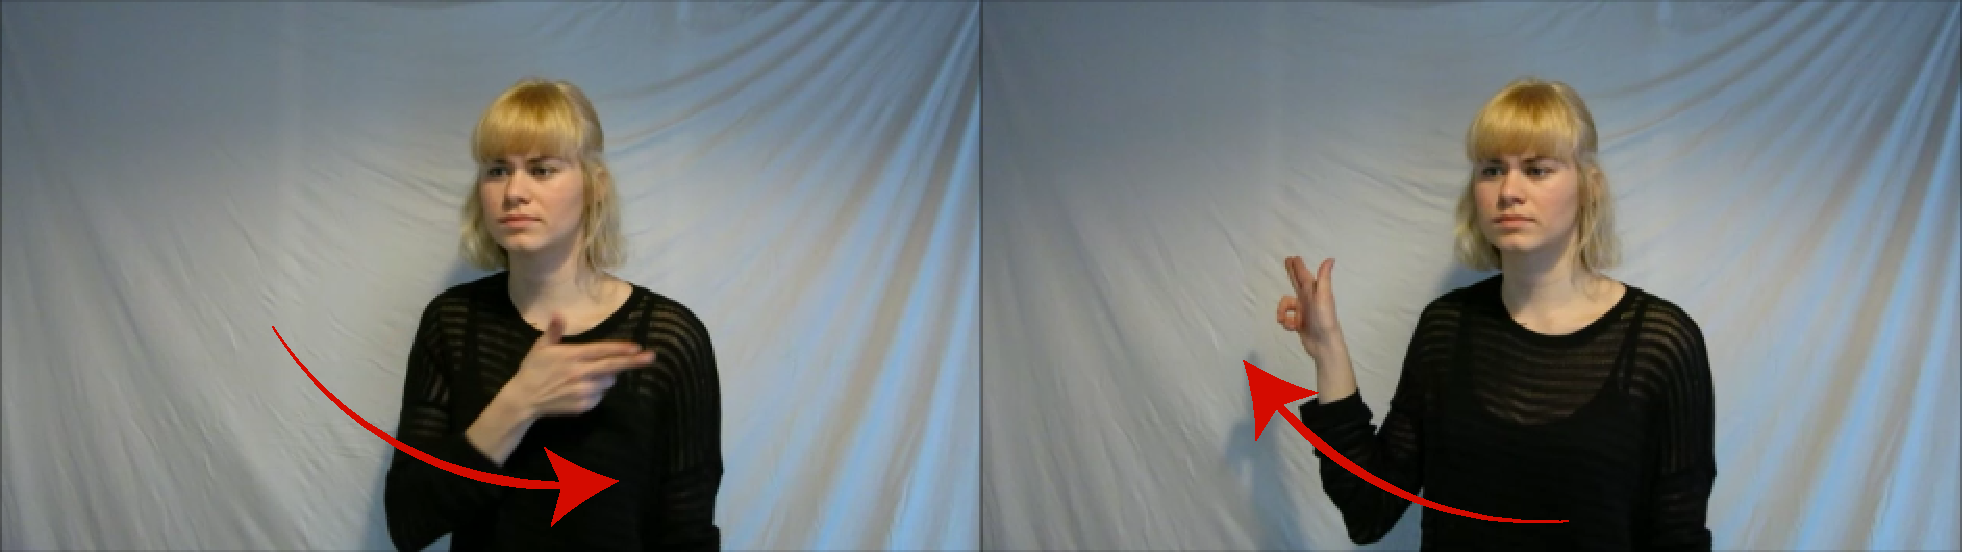
\includegraphics[resolution=300,width=0.9\textwidth]{Test1/Gestik-par/Gestik5_SkiftSang}
	\caption{Illustration af gestik-par 5; swipe med pege- og langefinger fra højre mod venstre for at skifte til det næste musiknummer og fra venstre mod højre for at skifte til det forrige musiknummer.}
	\label{fig:GestikPar5Skift}
\end{figure}
\noindent
%
Selvom gestik-par 5 kun er tildelt en første plads 3 gange, så indgår gestik-par 5 i testpersonernes samlede top tre ligeså ofte, som gestik par 1, jævnfør \autoref{tab:GestikParITopTreSkiftOversigt}. Gestik-par 5 er illustreret på \autoref{fig:GestikPar5Skift}. Testperson 9 giver udtryk for at de gestik-par, som indgår i top tre'en, er valgt ud fra hvad testpersonen kunne huske og hvad der så mest elegant ud. I relation til gestik-par 5 kommenterer testperson 9 at det virkede mest logisk, men at det samtidig virkede pistol-agtigt og at der var noget pege over det, uden at det blev et underviser-peg, hvor underviser-peget vurderes til at være negativt, jævnfør \autoref{fig:GestikPar5Skift}. Testperson 11 giver udtryk for at de gestik-par, som indgår i top tre'en er valgt ud fra hvad der er mindst naturligt i en samtale, hvorfor testpersonen har rangeret gestik-par 5 på en første plads. I forhold til gestik-par 5 vurderer testperson 11 at det giver intuitivt god mening at lave den bevægelse. Lignende synspunkter kommer til udtryk hos testperson 14, som igen vælger ud fra hvad der ikke føles naturligt og som testpersonen ikke vil komme til at lave ved en fejl, hvorfor et bestemt håndtegn er at foretrække. Desuden forbinder testperson 14 gestik-par 5 med en generel swipe-bevægelse, hvilket testpersonen finder naturligt. 

Tre ud af de syv testpersoner, testperson 1, testperson 2 og testperson 10, som har tildelt gestik-par 5, illustreret på \autoref{fig:GestikPar5Skift}, en anden plads gør det fordi det minder mest om gestik-par 1, illustreret på \autoref{fig:GestikPar1Skift}, som de alle tre har tildelt en første plads. Årsagen til at testperson 10 har rangeret gestik-par 5 på en anden plads er, udover at det minder om gestik-par 1, at det er nødvendigt at tænke mere over gestik-par 5 i forhold til gestik-par 1. Det vurderes at testperson 4 ligeledes vælger gestik-par 5 fordi det minder mest om testpersonens første plads; gestik-par 2, så i det her tilfælde vælges gestik-par 5 kun, hvis det fungerer efter samme princip som i gestik-par 2. Hos testperson 3 går lignende tendenser igen, hvor testpersonen har tildelt gestik-par 5 en anden plads, fordi parret er næstmest naturligt, hvor gestik-par 1 er mest naturligt. Dog kommenterer testpersonen at det giver mere mening at bruge to fingre til at flytte på noget, jævnfør \autoref{fig:GestikPar5Skift}. Udover at testperson 5 giver udtryk for at gestik-par 5 er mere feminin sammenlignet med gestik-par 1, hvilket er årsagen til at gestik-par 5 tildeles en anden plads, så pointerer testpersonen, at gestik-par 5 tillader kontrol over hvad der skubbes til. Derudover tilføjer testperson 5 at gestik-par 5 er mindre voldsom og nemmere at udføre siddende end gestik-par 1. Testperson 13 giver udtryk for at fortrække gestikker hvor der både er bevægelse og hvor hånden skal være i et bestemt tegn, jævnfør \autoref{fig:GestikPar5Skift}, hvilket formentligt er årsagen til at gestik-par 1 ikke fremgår på top tre'en, jævnfør \autoref{tab:GestikParITopTreSkift}. Testperson 15, som har tildelt gestik-par 5 en tredje plads, giver udtryk for at gestik-par 1 er logisk og havde et mere simpelt tegn end de andre forslag. 

Af de 12 gange gestik-par 5 indgår på en top tre er der fire testpersoner, som ikke også har inkluderet gestik-par 1. Fokuseres der på hvad de fire testpersoner ellers har inkluderet i deres top tre, så er det kun testperson 4, som har inkluderet en statisk bevægelse; gestik-par 3, de tre andre har alle inkluderet gestik-par med en eller anden form for swipe-bevægelse, jævnfør \autoref{tab:GestikParITopTreSkift}. Endvidere er der kun fem testperson ud af de 12, som har inkluderet gestik-par 5 i deres top tre, som også har inkluderet en statisk gestik; gestik-par 3, illustreret på \autoref{fig:GestikPar3Skift}, og når det er tilfældet rangeres gestik-par 5 altid højere. Med udgangspunkt i det, samt testpersonernes udsagn så tyder det i høj grad på, at de fortrækker bevægelse, særligt en swipe-bevægelse som forbindes med interaktionen på en tablet eller en smartphone, såfremt der skal skiftes musiknummer. Derudover tyder det på at en af de største årsager til at testpersonerne hyppigst tildeler gestik-par 5 en anden plads er fordi det minder mest om gestik-par 1.
%
\subsubsection{Forbedringsforslag til gestik-par 5}
\label{TestresultaterValgAfGestikkerForbedringGP5Skift}
%

To af de tre testpersoner, som har tildelt gestik-par 5 en første plads, har givet et forbedringsforslag. Testperson 9 foreslår at bevægelsen laves med tre fremfor to fingre, for at undgå et pistolagtigt udtryk. Problemet ved at gøre det med tre fingre er, at det for nogen er svært og ubehageligt at strække ringefingeren samtidig med at lillefingeren skal bøjes, hvorfor dette forbedringsforslag afvises. Testperson 11's forbedringsforslag anses, ligesom ved gestik-par 1, som værende en selvfølge; forbedringen ifølge testperson 11 er at bevægelsesmængden reduceres så det eksempelvis er muligt at skifte musiknummer med en swipe-bevægelse fra håndleddet.


%
\subsection{Valg af gestik-par til at skifte musiknummer}
\label{TestresultaterValgAfGestikkerValgSkift}
%
Baseret på foregående analyse samt \fullref{app:TestresultaterSkiftDaarlig} hvor i alt fem gestik-par er ekskluderet, så står valget mellem gestik-par 1 og gestik-par 5. Fælles for de to gestik-par er, at de indgår lige mange gange i testpersonernes samlede top tre; 12 gange i alt, selvom gestik-par 1 indgår 10 gange på en første plads og gestik-par 5 kun indgår tre gange. Det tyder på at de testpersoner, som har rangeret gestik-par 1 over gestik-par 5 giver udtryk for, at der egentlig ikke er så stor forskel mellem de to og at årsagen til at gestik-par 5 tildeles en anden plads frem for de resterende forslag skyldes at det minder mest om gestik-par 1. Derudover pointere flere testpersoner, som ikke nødvendigvis har rangeret gestik-par 1 over gestik-par 5, at de foretrækker dels, at gestikken indeholder en bevægelse og dels, at der er knyttet et bestemt håndtegn til gestikken. Ydermere er der flere testpersoner, som begår fejl når de udfører gestik-par 1, hvorimod ingen testpersoner begår fejl når de udfører gestik-par 5. Endvidere påpeger flere testpersoner at bevægelsen i gestik-par 1 er naturlig, hvorfor det antages at bevægelsen formentlig forekommer i ubevidst i deres kropssprog. I tillæg vurderes det, at størstedelen af de egenskaber testpersonerne foretrækker ved gestik-par 1 går igen i gestik-par 5. Tages alt dette i betragtning vurderes det, at der er belæg for at knytte gestik-par 5 til at skifte musiknummer.          

